\chapter{Mirrors for X-rays}
\label{capitolo2}
\thispagestyle{empty}

\begin{quotation}
{\footnotesize
\noindent{\emph{``Terence: Tu lo reggi il whisky? \\
Bud: Beh, i primi due galloni si, al terzo divento nostalgico e ci pu\`o scappare la lite... E tu lo reggi? \\
Terence: Eh, che domande, io sono stato allattato a whisky!''
} }
\begin{flushright}
I due superpiedi quasi piatti
\end{flushright}
}
\end{quotation}
\vspace{0.5cm}

\noindent As discussed in Chapter \ref{capitolo1}, to have focusing properties for X-ray radiation, refraction optics are useless, due to the strong interaction with matter of X-rays. Thus reflection optics, at grazing incidence angle to have a good signal is needed. Mirrors that carry out any focusing must have a curved surface. A Working at normal incidence, it is possible to obtain a form a good image using a concave mirror. But this is not the case for X-ray that work, as said before, at grazing angle, this introduce some kind of optical aberration.A spherical surface has the property that the rate of change of the surface slope is exactly the same everywhere on the surface, and thus the aberration is inevitable. This shape bring an intrinsic aberration ("spherical aberration").
If the slope in not any more constant all over the mirror but become flatten in the region surrounding the outer rays, it is possible to focus all the rays in the same point. While correction of spherical aberration is not the only application of aspherical surfaces, it is one of the major application areas.

\section{Spherical surface}
\noindent To define a spherical surface is needed only the radius of curvature.  A spherical surface is defined by only one parameter, the radius of curvature of the surface. 
\subsection{Astigmatism}
In Figure \ref{fig: System1} it is showd an image formation of a beam with a spherical mirror with radius $R $, at grazing incidence $\theta_i $, with a divergence $\beta $ from the point source P. The oject length $u $ is equal to the distance PO and the image distance $v $ correspond to OQ.
\begin{figure}[]
%
\centering
%
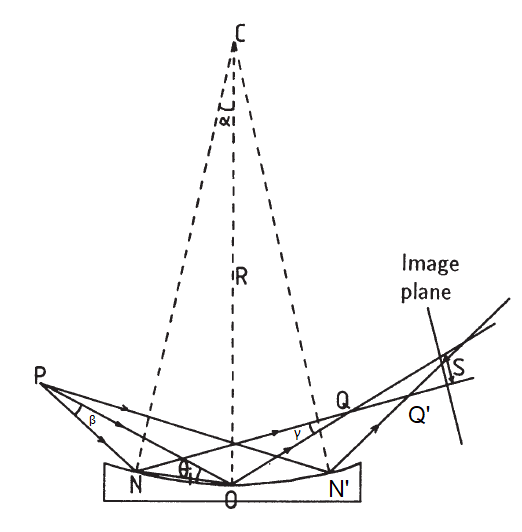
\includegraphics[width=.6\textwidth]{Immagini/Chapter2/System1}
%
\caption{Formation image of a circular mirror}
%
\label{fig: System1}
%
\end{figure}
\noindent The beam hit the mirror over a distance equal to $k = $ NO, such as $k<<R $, that correspond to a small divergence $\beta $. The cord NO subtends an angle $\alpha $ with the center of the sphere C, thus $k = R \alpha $, $\gamma $ is the convergence angle of the beam at the focal point Q. For small angle approximation, from the triangle PNO ,
\begin{equation}
\beta = R \alpha \frac{\theta_i - \alpha / 2}{u - R \alpha}
\label{eq: beta}
\end{equation}
\noindent and from QNO
\begin{equation}
\gamma = R \alpha \frac{\theta_i + \alpha / 2}{v + R \alpha}
\label{eq: gamme}
\end{equation}
\noindent The reflection law impose that $\beta + \gamma = 2 \alpha$, thus:
\begin{equation}
\frac{1 - \alpha / (2 \theta_i)}{u - R \alpha} + \frac{1 + \alpha / (2 \theta_i)}{v + R \alpha} = \frac{2}{R \theta_i}
\label{eq: refle lae}
\end{equation}
\noindent in case of paraxial approximation
\begin{equation}
\frac{1}{u} + \frac{1}{v} = \frac{2}{R \theta_i} = \frac{1}{f_m}
\label{eq: reflection law}
\end{equation}
\noindent where
\begin{equation}
f_m = \frac{R \sin \theta_i}{2}
\label{eq: fm}
\end{equation}
\noindent that it reduce to $f_m = \frac{R \theta_i}{2} $ for small angle, $f_m $ is named meridian focal length. 
\\
In case of a three dimensional spherical mirror, a second image is generated, as it is showed if Figure \ref{fig: MeridianAndSagittal},with a focal distance equal to:
\begin{equation}
f_s = \frac{R}{2 \sin \theta_i}
\label{eq: fs}
\end{equation}
\noindent and it is named sagittal focal length.
\begin{figure}[]
%
\centering
%
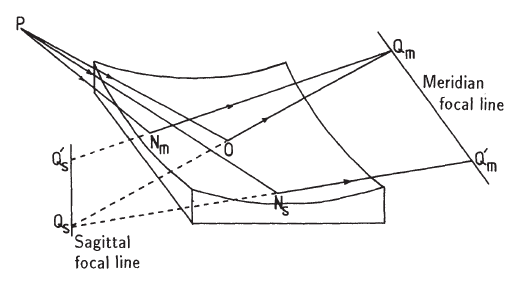
\includegraphics[width=.6\textwidth]{Immagini/Chapter2/MeridianAndSagittal}
%
\caption{Image formation of a 3D spherical mirror}
%
\label{fig: MeridianAndSagittal}
%
\end{figure}
\noindent For Figure \ref{fig: MeridianAndSagittal} it is possible to note that the two image for a point wise source are lines, where the meridial line is in the plane of the mirror and the sagittal line perpendicular to it. Equation \ref{eq: fm} and Equation \ref{eq: fs}, are equal for incidence angle $\theta_i = 0^{\circ} $ . In the case of grazing incidence the situation is bad, for example, with a $\theta_i = 2^{\circ} $, the sagittal focal length is $10^3$ times the meridial length.
\subsection{Spherical Aberration}
Spherical mirror are also affected, as it is showed in Figure \ref{fig: System1}, by a transverse spherical aberration. This aberration can be determined relating it with the the variation of $v $ with $\alpha$:
\begin{equation}
S = \Delta v \sin \gamma \simeq \Delta v \gamma
\label{eq: S}
\end{equation}
\noindent where S is the coefficient that determine the spherical aberration. Moreover, from Equation \ref{eq: refle lae}, in case of $\alpha =0 $:
\begin{equation}
v_0 = \frac{f_m u}{u - f}
\label{eq: v0}
\end{equation}
\noindent otherwise:
\begin{equation}
v = v_0 + \Delta v = f_m u - \frac {\frac{3 u R \alpha}{4} + \frac{R^2 \alpha^2}{2}}{u - \frac{3 R_{\alpha}}{4} - f_m}
\label{eq: v}
\end{equation}
\noindent defining a magnification such as
\begin{equation}
M = \frac{v}{u}
\label{eq: M}
\end{equation}
\noindent combining it with Equation \ref{eq: beta} and Equation \ref{eq: gamme}
\begin{equation}
\gamma = \frac{2 \alpha}{M + 1}
\label{eq: new gamme}
\end{equation}
\noindent So
\begin{equation}
S = \frac{3 R \alpha^2}{2} (M + 1) = \frac{3 k^2}{2 R} (M + 1)
\label{eq: new S}
\end{equation}
\noindent the dependance of S with respect to k is quadratic, so all the rays are deviated to the same side of $\alpha = 0$ image point.
\subsection{Reducing aberration}
For spherical mirror it is possible to reduce the aberration using large grazing angle (decrease astigmatism) and small aperture (decrease spherical aberration). For the first solution it have to consider the total external reflection, so it have to choose a material that have a big value of the critical angle $\theta_c $. An example can be the Carbon that have a critical angle of $\theta_c = 18^{\circ} $ for $K_{\alpha} $ radiation, this correspond to have a ratio $f_s $ over $f_m $ of $11 $, that is still big.
\\
Reducing the aperture it means to reduce $k $, it is reduce also the spherical aberration but also the collecting power of the mirror. This is bad because the resolving power is limited by the diffraction limit that is $\simeq \frac{\lambda}{2 \theta} $, where $\theta $ is the maximum semiaperture, that, for grazing angle, correspond to $\theta_i $.

\section{Conic Surfaces}
As said before, to go beyond the spherical mirror correcting the aberration, there exist aspherical surfaces that are defined with more than one parameter, in general by an analytical formula. The easier aspherical surface is the toroidal surface, a surface that is defined with two radii of curvature, the meridian one $R_m $ and the sagittal one $R_s $. A particular choice of radii can be
\begin{equation}
R_m \sin \theta_i = \frac{R_s}{\theta_i}
\label{eq: toroidal 1}
\end{equation}
\noindent in such a way to have equal focal length and so no asytgmatism. Thus
\begin{equation}
R_s = R_m \sin^2 \theta_i
\end{equation}
Other kind of aspherical surfaces are those named $"conic surfaces"$ that can be defined as

\begin{equation}
	z = \frac{c r^2}{1 + \sqrt{1 - (1 + k)} c^2 r^2}
\end{equation}

\noindent where $c $ is the base curvature at the vertex, $k $ is a constant that define the kind of conical surface, and $r $ is the radial coordinate of the point on the surface. In Table \ref{tab: conic surface}, and in Figure \ref{fig: SurfaceConic1} is showed the relation between the $k $ constant and the kind of surface

\begin{table}[ht]
	\centering
		\begin{tabular}{l|r}
			Conic Constant k & Surface Type\\
			\hline
			0 & Sphere \\
			$k < -1 $ & Hyperboloid \\
			$k = -1 $ & Paraboloid \\
			$-1 < k < -0 $ & Ellipsoid \\
			$k > 0 $ & Oblate Ellipsoid \\	
		\end{tabular}
	\caption{Parameter of different conic surfaces}
	\label{tab: conic surface}
\end{table}
\begin{figure}[]
%
\centering
%
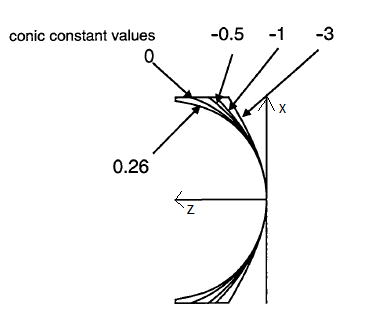
\includegraphics[width=.4\textwidth]{Immagini/Chapter2/SurfaceConic1}
%
\caption{Different kind of surface conic, with the same $c $ base curvature value, and different constant $k $.}
%
\label{fig: SurfaceConic1}
%
\end{figure}
\noindent A good point that have the conical surfaces are the no-presence of spherical aberration. As said in before, spherical surface affected buy spherical aberration if the configuration is different from the normal incidence. The ellipsoidal geometry forms create a free-aberration image for a couple of real object on the same side of the surface, on the contrary the hyperbola work for conjugates on different side of it. Parabolic surface create a perfect image for any axial object place at infinity, this is the reason why parabolic mirror are very used for astronomical application. For all the shapes of surfaces, if the object is moved from it's ideal position aberration will appear: an axial movement introduce a certain amount of spherical aberration, lateral movement introduce other types of aberration such as coma, astigmatism and field curvature.
\\
\noindent The importance of aspherical surface for mirror consist in the fact that, differently from the lenses, is not possible to build a spherical surface with different radii, in the lenses case it different spherical radii, and so, aspherical surface, serve to minimize the aberration. 
Figure \ref{fig :spher abb corr} show a simple example of how it is possible to correct the spherical aberration using a paraboloid mirror \ref{fig: ParabolicMirror} instead of a spherical mirror \ref{fig: Sphericalmirror}
\begin{figure}[]
%
\centering
%
\subfloat[][Spherical mirror \label{fig: Sphericalmirror}]
   {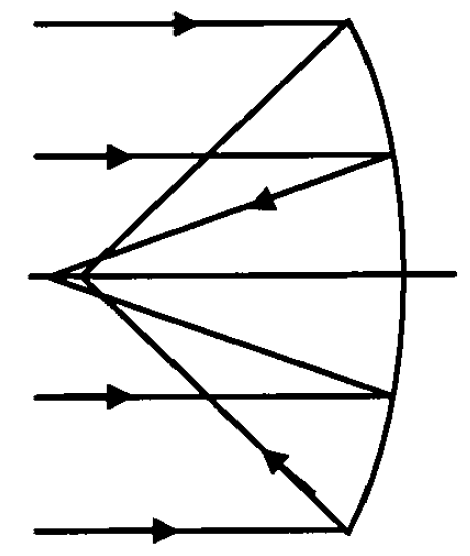
\includegraphics[width=.2\textwidth]{Immagini/Chapter2/SphericalMirror}}\quad
%
\subfloat[][Parabolic Mirror  \label{fig: ParabolicMirror}]
   {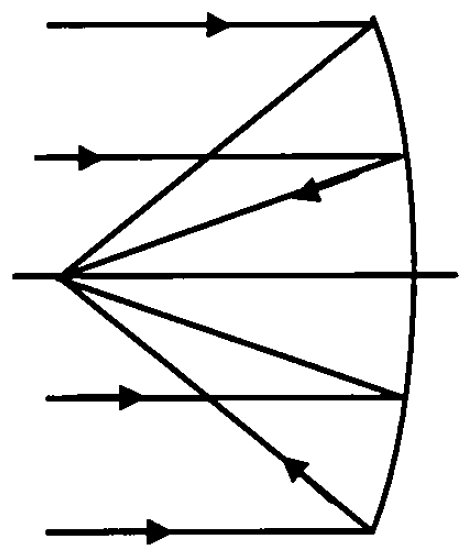
\includegraphics[width=.2\textwidth]{Immagini/Chapter2/ParabolicMirror}}
%
\caption{Example of spherical aberration correction}
\label{fig :spher abb corr}
%
\end{figure}

\section{Compound Optical system}
An optical system designed to obtain an image that reproduce correctly the object image must satisfy the Sine-Abbe condition
\begin{equation}
\frac{sin u^{'}}{sin U^{'}} = \frac{sin u}{ sin U}
\label{eq: SineAbbe}
\end{equation} 
\noindent where, as it is showed in Figure \ref{fig: SineAbbe}, $u $ and $u^{'} $ are rays that leave the object, $U$ and $U^{'} $ are the angles of the same rays that reach the image plane. In other world, the sine of the ray that leave the object must be proportional to the sine of the angles that reach the image plane.
\begin{figure}[]
%
\centering
%
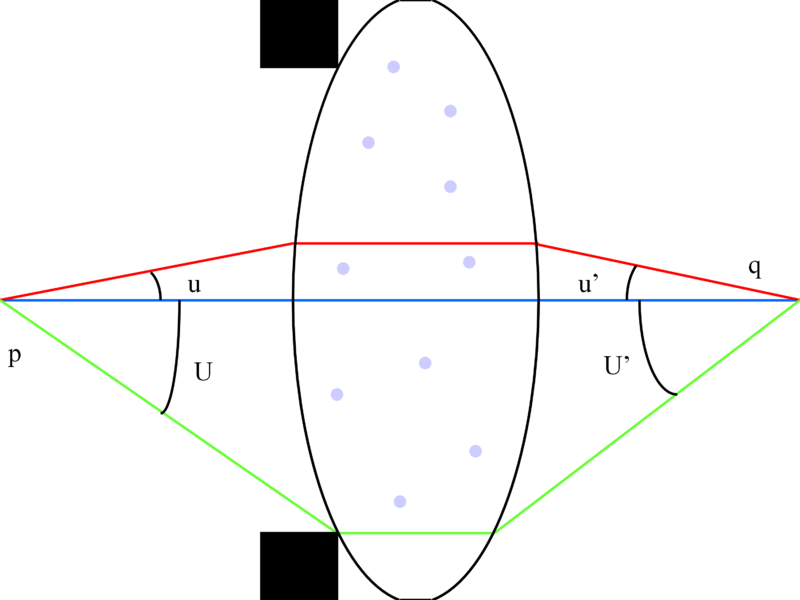
\includegraphics[width=.6\textwidth]{Immagini/Chapter2/SineAbbeCondition}
%
\caption{Sine Abbe condition for a lens}
%
\label{fig: SineAbbe}
%
\end{figure}
Unfortunately, for the case of mirror, there is no way to satisfy the Sine Abbe condition using only one mirror. To satisfy the condition, and so obtain a better image, there are invented optical system composed by more than one mirror. The system that whose invented which respect the condition are the Wolter system, widely used in astronomy, that use a combination of coaxial and confocal conic section.A first approximation system that respect the sine Abbe condition are the Kirkpatrick-Baez system and Montel or nested-Kirkpatrik-Baez system, those compound optical system involves reflector whose meridian planes are at right angle (crossed).
\subsection{Wolter System}
\hspace{10mm} In 1952 Wolter published a paper in which he discussed several disposition of two conical mirror in order to collect light for an astronoical use. Figure show the different disposition discussed: Wolter $\mathrm{I} $, Wolter $\mathrm{II} $, Wolter $\mathrm{III} $.
\noindent Wolter $\mathrm{I} $ telescope consist of a coaxialparaboloid (primary mirror) and hyperboloid (secondary mirror). The focus of the paraboloid is coincident with the rear focus of the hyperboloid, and the reflection inside both mirrors. The Wolter $\mathrm{II} $ telescope use the same kind of mirror of Wolter $\mathrm{I} $ paraboloid and hyperboloid. But the focus of the paraboloid coincident with the front focus of the hyperboloid, and, the reflection, occurs internally for the paraboloid and externally for the hyperboloid. The Wolter $\mathrm{III} $ telescope consist in a paraboloid and an ellipse. In this system the first mirror is the paraboloid one, and the second is the ellipsoidal that have front focus coincident with that of the parabola, moreover the reflection is external for the paraboloid and internal for the ellipsoidal.
\noindent The Wolter $\mathrm{I} $ have typical grazing angle of less than a degree and is used for hard X-rays. The Wolter $\mathrm{II} $ telescope has typical grazing angle of, approximate, 10 degree and is used for soft X rays and extreme ultraviolet (EUV).
\noindent Because of circular symmetry, astigmatism and spherical aberration are eliminated but  exhibit coma aberration. Other problem is the difficulty of fabrication , and require a huge area to achieve a very small collecting angle.
\begin{figure}[]
%
\centering
%
\subfloat[][Wolter I  \label{fig: Wolter1}]
   {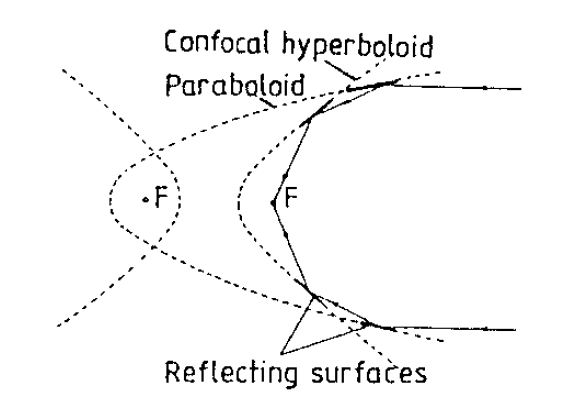
\includegraphics[width=.4\textwidth]{Immagini/Chapter2/Wolter1}}
%
\subfloat[][Wolter II \label{fig: Wolter2}]
   {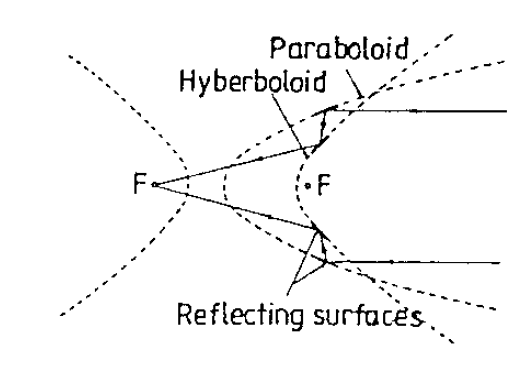
\includegraphics[width=.4\textwidth]{Immagini/Chapter2/Wolter2}}\quad
%
\subfloat[][Wolter III  \label{fig: Wolter3}]
   {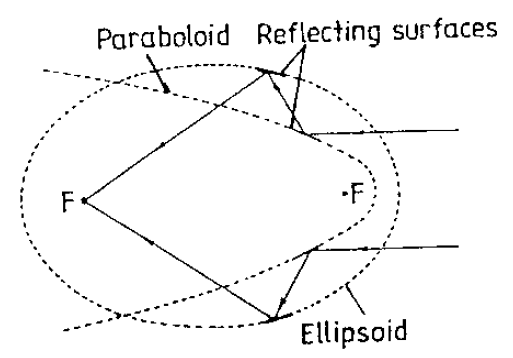
\includegraphics[width=.4\textwidth]{Immagini/Chapter2/Wolter3}}
%
\label{fig :Wolter Systems}
%
\end{figure}

\subsection{Kirkpatrick-Baez System}

\hspace{10mm} This kind of optics are used in the ESRF and consist, as shown in Figure, in two separated cylindrical surface conical mirror that focus the incident beam in both saggital and transverse thus astigmatism is removed. Although such system introduce another type of distortion, anamorphotism. Because of the different distance of the image plane with respect to the mirrors the magnification is different in the two direction.  Another technical problem that face with system is the big volume that occurs to implement it.
\noindent To overcome those two problem and obtain a system that conjugate the good behaviour of the KB system with an equal magnification of the two direction and compact system, it is possible to implement a system as it is showed in Figure, a system in which both mirrors are at the same distance from the object. This sort of arrangement is extremely difficult to manufacture and, consequently, very expensive.
\noindent Despite these problem K-B system are very used in ESRF and in European synchrotron, on the contrary, in American synchrotron another type of optical system, named "Montel", is used that will be discussed in the next section.
\begin{figure}[H]
%
\centering
%
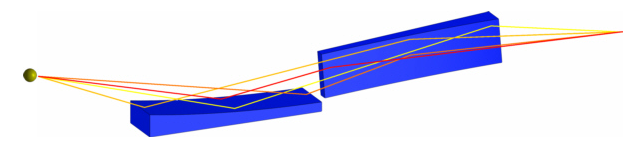
\includegraphics[width=.6\textwidth]{Immagini/Chapter2/KBSystem}
%
\caption{Different kind of surface conic, with the same $c $ base curvature value, and different constant $k $.}
%
\label{fig: SurfaceConic1}
%
\end{figure}


\section{Montel}

\hspace{10mm} As discussed before KB system have some limitation that can be overcome with a different optical system named "Montel". This geometry bring four important advantages for high-precision focusing: 
\\ i) the optical system is more compact which allow greater working space;
\\ ii) the focal distance of the two mirror are the same, this cancel out  the anamorphotism;
\\ iii) the alineation of the system is easier with respect to the KB system because, in this case, only one thing has to be aligned, however , in the KB there are two separated mirror that has to be aligned;
\\ iv) the divergence that can be collected is larger which allows for greater flux and/or a lower diffraction limit.
\begin{figure}[H]
%
\centering
%
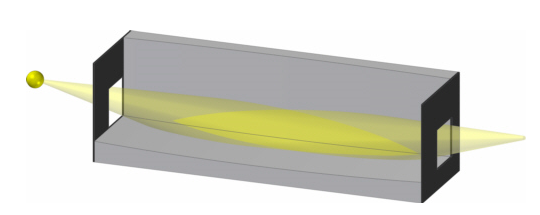
\includegraphics[width=.6\textwidth]{Immagini/Chapter2/MontelSystem}
%
\caption{Different kind of surface conic, with the same $c $ base curvature value, and different constant $k $.}
%
\label{fig: SurfaceConic1}
%
\end{figure}

\subsection{Diffraction limit of Montel compared to sequential K:}
The image quality and dimension, for x-rays reflective optics, is  caused by aberration, mirror imperfection, and magnification of the system. Nowadays it is possible to create a mirror with high surface quality with a so high demagnification that the spot focal size is limited,p primary, by diffraction and mechanical/environmental factors.
\begin{figure}[H]
%
\centering
%
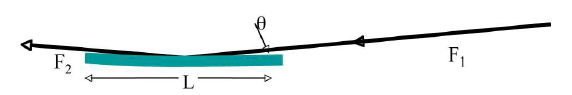
\includegraphics[width=.7\textwidth]{Immagini/Chapter2/System3}
%
\caption{Different kind of surface conic, with the same $c $ base curvature value, and different constant $k $.}
%
\label{fig: System3}
%
\end{figure}
The first limiting factor (diffraction) depends on the wavelengths of the radiation and on the divergence of the Beam. Figure \ref{fig: System3} show a simple elliptical mirror with an object focal of $F_1 $, an image focal of $F_2 $, an incidence angle $\theta $ and a length of the mirror equal to $L $. For piraticpraticalal calculation it is convenient to use the system in Figure \ref{fig: System4} , where $F_d $ is the distance from the end of the mirror to the image focal, $\theta_i $ the divergence focused at the image point, $\theta_d $ the maximum accepted angle, $\theta_o $, the divergence intercepted by the mirror.
\\
For an elliptical KB system the FWHM of the diffraction limit in each plane is:
\begin{equation}
D_{FWHM} \sim  \frac{0.88 \lambda}{\theta_i}
\label{eq: D_FWHM}
\end{equation}
\noindent where $\lambda $ is the wavelength of the radiation. For the total external reflection that rules the reflection for the X-ray, the maximum divergence that can be collected is that which correspond to the critical angle $\theta_c $, that can be calculated as
\begin{equation}
\theta_c \sim \sqrt{\rho \delta} = 6.7 10^{-2} \lambda (nm) = \frac{8.4 10^{-2}}{E(keV)}
\label{eq: theta_c}
\end{equation}
\noindent In reality, due to geometrical constrain on sequential KB system, the maximum divergence that can be collected is about $0.84 \theta_c $.
\begin{figure}[H]
%
\centering
%
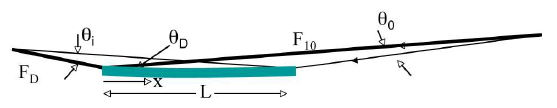
\includegraphics[width=.7\textwidth]{Immagini/Chapter2/System4}
%
\caption{Different kind of surface conic, with the same $c $ base curvature value, and different constant $k $.}
%
\label{fig: System4}
%
\end{figure}
%
To study the diffraction limit of a KB system, it is done a theorical treatment of micro focusing using elliptical mirror, and working on the parameter that define the geometrical shape, using the system in Figure \ref{fig: System4}. The image and objective divergence, $\theta_i $ and $\theta_o $, depend on the angle $\theta_d $, the ratio $L $ over $F_d $, length of the mirror over the distance between the image focus and the end of the mirror, and the angle $\theta_d $.
\begin{figure}[]
%
\centering
%
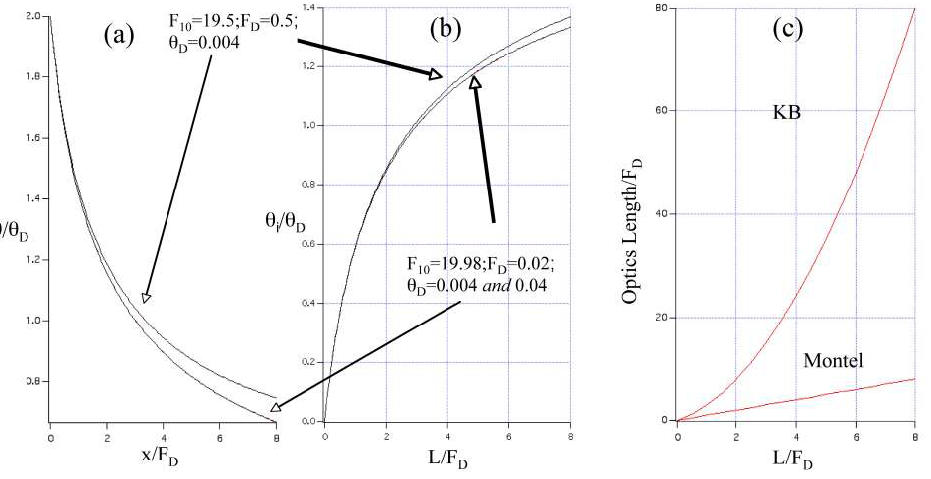
\includegraphics[width=1.\textwidth]{Immagini/Chapter2/Plot1}
%
\caption{Plot1}
%
\label{fig: Plot1}
%
\end{figure}
%
\noindent Figure \ref{fig: Plot1} can be used to estimate the fraction of the mirror that can reflect different wavelengths. If the mirrpr is designed to work for the wavelength $\lambda $ with $\theta_d = \theta_c $, a new wave with wavelength equal to $\lambda / 2 $, the part of the mirror that is covered is that with $x / F_d > 3.5$ reflect efficiently the radiation. With Figure \ref{fig: Plot1} b it is possible to estimate the radiation collect at the image plane. Normalizing the length of the mirror with $F_d $ and, normalizing the divergence angle collected with the biggest angle $\theta_d $, then the normalized numbers fall down to a universal curve aass menobhysa di a foactor of 10-20. This curve is useful because it can estimate the radiation collected by the KB/Montel.For example, if $L/F_d $ is n for each mirror of the KB system, then the total length of the system is related to the clearance distance of the second mirror
\begin{equation}
L= (2 n + n^2 ) F_d
\label{eq: clearance distance}
\end{equation}
\noindent for the Montel system the total length is only $L = n F_d $. In Figure \ref{fig: Plot1} c is showed the length of both compound system, and, for large  $n>2 $ the situation is dramatical, for example for $n=2 $ KB length is about the same of Montel with $n=8 $. This mean that the diffraction limit for total external reflection for KB is about $16 nm$, for Montel $11 nm$.
\\
Mirrors can be designed to work well with short or medium or large wavelengths. Depending on the design, the diffraction  limit is limited to certain conditions. If the mirrors are designed for short wavelength, according to Equation \ref{eq: D_FWHM}, the diffraction limit is mainly governed by the wavelength, because the divergence collected is roughly independent from the wavelength. On the contrary, if the mirror are optimized to long wavelengths, the surface that reflect the radiation is only a fraction, this compromise the shortest wavelength. Figure \ref{fig: Plot2} show the dependace of the diffraction limit with mirror designed to be optimize, with the choice of the $\theta_d $ to different situation.
%
\begin{figure}[]
%
\centering
%
\subfloat[][Plot2 \label{fig: Plot2}]
   {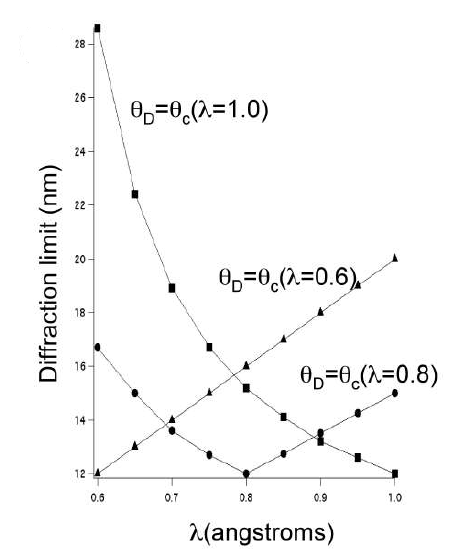
\includegraphics[width=.5\textwidth]{Immagini/Chapter2/Plot2}}
%
\subfloat[][Plot3  \label{fig: Plot3}]
   {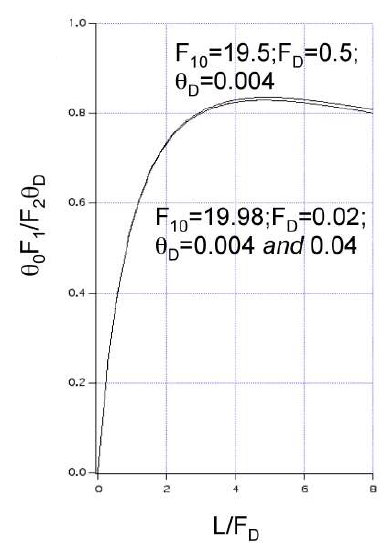
\includegraphics[width=.5\textwidth]{Immagini/Chapter2/Plot3}}
%
\caption{Plots}
\label{fig :Plots}
%
\end{figure}
%
\subsection{Flux limit}
If the beam is small, the flux is the limitating factor to the image spot. For the KB optics designed to demagnify the source, increasing the length of the mirror than the collected divergence increase, the backdraw is that the demagnification decrease, in the sense that became less strong, so, to reobtaine the desired image dimension it have to decrease the object spot. The geometrical demagnification is, according to Figure \ref{fig: System4},
\begin{equation}
\frac{F_d (1 + n / 2 )}{F_10 - n F_d / 2} =\frac{F_2}{F_1}
\label{eq: geometrical demag}
\end{equation}
\noindent and the collect divergence of the radiation at the image plane is $\theta_0 $. As it is reported in Figure \ref{fig: Plot3}, the performance fall down to another universal curve for large and small demagnification.
\\
In this case the Montel system is better than the KB optics because of the largeer numerical aperture that increase the flux on the sample. This last point is convenient for neutron experimental uses where the flux limit overcame the diffraction limit, differently than the X-ray experiments. Montel flux is 2.6 times increase with respect to the KB. A Montel long $0.25m $ of clearance has $n = 2 $, a similar value to the longest of the mirror give an $n \sim 0.73 $, with a difference in the total flux collect into a small spot of $\sim 2.5$.
\subsection{Optical Design}

The mirrors used in this Montel configuration are mirror that have a cylindrical shape in one direction and elliptical shape in the other direction. One approach to obtain the Montel system is that to use two pre-figured elliptical mirror and grind the cut site at 45$^\circ $ as shown in figure. After that it place the mirrors together makes a good fit with no gap requiring no contouring of the mirror side. Another way involves diveding pre-figured elliptical mirror into two part that, add them together, can form the Montel system. This approaches is primary driven by the fact that in a conventionally polished mirror, the clear aperture area has the best figure and finish. As such uAs such, using two halves of a prefigured mirror cut in the middle has several advantages- including consistency and economy. There are major challenges
however. First, the mirror surface must be protected against damage and deformation during cutting and subsequent figuring operations. After cutting into two, the cut sites must be treated (e.g., etched) to remove any subsurface damages that could alter a mirror's figure. Then the mating side of one of the mirrors must be contoured and polished such that when it is placed against the partner mirror, it makes a nearly perfect fit with good surface quality all the way to the contact edge.This last two-steps are crucial because if there is a significant gap or if the mirror surfaces in the vicinity of the interface are damaged, a significant part of the incident beam could be lost. As an example, we are developing a pair of Montel mirrors for polychromatic nanofocusing on Sector 33 at APS. This beam line will use 40 mm long elliptical mirrors for nano-focusing a 100 $\mu m$ beam to a 50 nm spot at 2000x demagnification. This concave elliptical mirror has a maximum depression of about 6 $\mu m$ at its center. If cut flat and placed against its mating mirror, a gap as large as 6 $\mu m$ is created which loses about 10$\% $ of the 100 $\mu m$ incident beam. Similarly, if the mirror surfaces near the intersection are damaged, then beam loss can be significant.
\begin{figure}[]
%
\centering
%
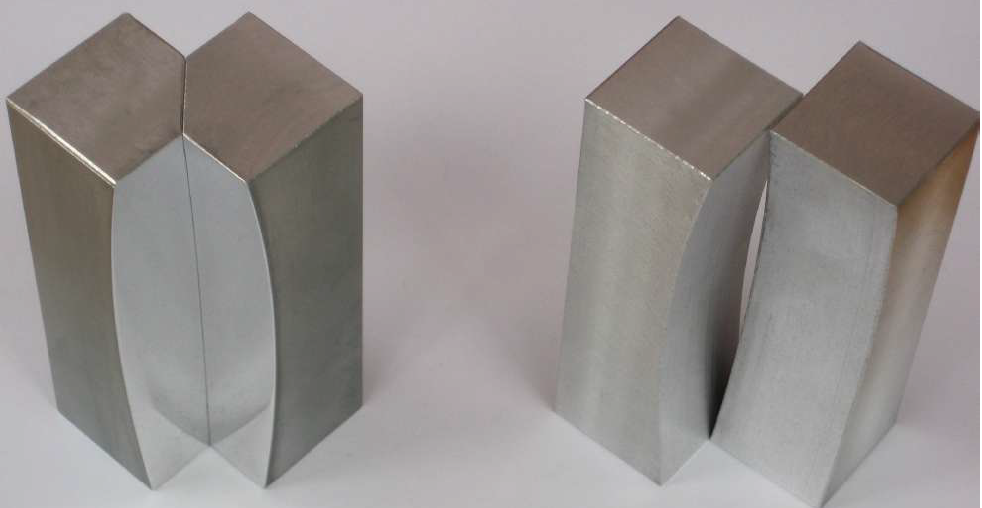
\includegraphics[width=.8\textwidth]{Immagini/Chapter2/MontelEdges}
%
\caption{Different kind of surface conic, with the same $c $ base curvature value, and different constant $k $.}
%
\label{fig: MontelEdges}
%
\end{figure}
